\documentclass[twoside,single]{lion-msc}
\usepackage{lipsum}


\title{Identifying the molecular diagnostics from disk models to infer the elemental abundances and disk substructures in JWST spectra}
\author{Niels de Klerk}

\major{Astronomy and Physics}
\affiliation{Leiden Observatory, Universiteit Leiden}

\newdate{date}{\day}{\month}{\year}           % definition of time and date using datetime package
% \newdate{date}{27}{08}{2010}
\date{\displaydate{date}}

\studentid{s3640477}                           % check you student ID, LaTeX does not do this
\abstract{Here goes a wonderful abstract.}   % limit your self to 1/2 page or 500 words
\dailysupervisor{Msc. Marissa Vlasblom \\ \hspace*{\fill}Msc. Aditya Arabhavi}
\supervisor{Prof. Dr. Ewine van Dishoeck \\ \hspace*{\fill}Prof. Dr. Inga Kamp} % Note that this should be a LION staff member!
\corrector{Dr. Matthieu Schaller}                      % This could be a LION staff member or your external supervisor

\degree{Bachelor of Science}                     % The default option is "Bachelor of Science", change if needed

\major{Astronomy and Physics}                  % The default option is "Physics", change if needed
%\major{Physics and Mathematics}

% optional cover picture - should be jpg or pdf
% \coverpicture{
\includegraphics[width=10cm]{Latex/lion-msc-logo.pdf}}

% Use this to make hyperlinks visible in the document.
% \hypersetup{colorlinks=true}

% ---------------------------------------------------------------- My defintions!
% \renewcommand{\vec}[1] {\ensuremath{ \overrightarrow{ #1 } }}
\renewcommand{\vec}[1] {\ensuremath{ \mathbf{ #1 } }}
% \bra \ket \braket and \proj
\newcommand{\bra}[1]{\ensuremath{\langle #1 \vert}}
\newcommand{\ket}[1]{\ensuremath{\vert #1 \rangle}}
\newcommand{\braket}[2]{\ensuremath{\langle #1 \vert #2 \rangle}}
\newcommand{\proj}[1]{\ensuremath{\vert #1 \rangle \langle #1 \vert}}

\newcommand{\kpar}{\ensuremath{k_\parallel}}
% ----------------------------------------------------------------

% \usepackage{tocloft}
% \renewcommand{\cftchapdotsep}{\cftdotsep}
\begin{document}

% roman numbering in the table of contents section
\pagenumbering{roman}

\maketitle

% Table of contents:  it is a good idea to include this into your thesis
\tableofcontents
\cleardoublepage
\pagenumbering{arabic}
\chapter{Introduction}
The nebular hypothesis was first proposed in \textit{The Principia} by Emanuel Swedenborg in 1745. Immanuel Kant developed the theory further in 1752 and it was modified by Pierre-Simon Laplace in 1796. The theory states that a planetary system is formed from a slowly rotating gas cloud, which collapses down into a disk. Centuries later, the first protoplanetary disk was observed by O'Dell using the Hubble Space Telescope \citep{ODell1993}. In recent years, the Atacama Large Millimeter/submillimeter Array (ALMA) has imaged a large collection of these protoplanetary disks showing a wide variety of structures and compositions. The JWST MIRI mid-INfrared Disk Survey (MINDS) team uses the JWST to investigate the inner parts of protoplanetary disks. The study of the protoplanetary disks is important to find answers to the fundamental questions, 'How did life arise?' and 'Are we alone in the universe?'.

The spectrum of protoplanetary disks can tell us a lot about the properties of the disk and the host star. An important example is an observation of the disk around a T Tauri star 89 sz\cite{Gasman_2023}. Using MIRI on the JWST they probed the inner regions of the disk. They detected CO$_2$, H$_2$O, OH, CO, and HCN. Furthermore, no other organics were detected, suggesting a low C/O ($<$0.5) ratio. This result was different from the ratio found using ALMA ($>$1) which probed the outer regions. This highlights the complexity of disks and their chemistry.

However, this observation is not necessarily representative of disks. \cite{colmenares2024jwstmiridetectioncarbonrichchemistry} observed a disk around the T Tauri star DoAr 33 with an exceptionally high C/O ratio of 2-4. In addition to CO, H$_2$O, and CO$_2$ like in the 89 sz disk the more complex carbohydrates C$_2$H$_2$ and C$_4$H$_2$ were found. The presence of these molecules is indicative of this high ratio. A possible explanation for this carbon-rich environment is the slow accretion rate of the star which results in slowing the radial mixing and the persisting of the carbon-grain destruction.

Observations of the protoplanetary disk around the T Tauri star GW lup have given the first detection of $^{13}$CO$_2$ in a protoplanetary disk. \cite{Grant_2023} The combination with the spectral resolution of the JWST-MIRI and the high SNR allows for the detection of weaker spectral features. Notably, the deduced N$_{CO_2}$/N$_{H_2O}$ was significantly higher than previously thought. This could indicate a cavity between the H$_2$O and CO$_2$ snowlines. These findings show the new possibilities JWST provides to study disk structures. 

The effects of a cavity on the spectrum were studied by \cite{vlasblom2023midinfraredspectrattauri}. It was speculated that 'CO$_2$-only sources' have inner cavities which extend beyond the H$_2$O snowline, but stay within the CO$_2$ snowline. By running thermo-chemical models with different inner cavity sizes it was shown that N$_{CO_2}$/N$_{H_2O}$ grows as the size of the cavity grows and then sharply drops. The conclusions drawn from this can help to interpret the spectra of disks.

In chapter \ref{Ch: Theoretical Background} we give background information about processes in the protoplanetary disks and simulations. We present the data and the methodology in chapter \ref{Ch: Methods}.



% \chapter{Theoretical Background}\label{Ch: Theoretical Background}
\section{Formation and evolution of Disks}
Molecular clouds are large collections of gas and dust. When these clouds are perturbed, parts of the cloud can become dense enough, making them collapse under their gravity. This will result in the creation of a star surrounded by gas and dust. The angular momentum of each of the particles is randomly oriented, but on average the angular momentum vector is pointed in a certain direction. Two particles colliding will cause them to exchange angular momentum. If many collisions happen, all the angular momenta of the other than the average angular momentum vector get canceled out. This results in the formation of a disk around the pre-main-sequence star.
The evolution of the disk can be categorized into 4 classes \cite{1987ApJ...312..788A}. Class 0 are objects where an optically thick envelope surrounds the protostar. Class I objects have a star and disk but are still embedded in an optically thick envelope. The star and disk become visible in class II objects as the star has become bright enough to blow away the envelope. In class III objects, the disk has largely been depleted of gas and dust, leaving behind planets and planetesimals. 
% Factors that influence the evolution


\section{Structure}
The protoplanetary disk has structure, namely the radial structure and the vertical structure. The innermost regions ($<$10 AU) of the disk are the hottest and receive the most radiation. Most of the molecules are in gaseous form in this region, except for some silicates and metals. The star heavily influences the chemistry. The intermediate regions (10-100 AU) have lower temperatures, allowing molecules like water to condense. The outer regions ($>$100 AU) are the coldest in the disk. Molecules have formed ice here making them inert. \\
The height of the disk is also an important factor in its structure. The midplane is the horizontal plane through the center of the disk. Most dust particles settle around the midplane whereas the gas particles are further out. The midplane is also colder than the outside of the disk as it receives less light from the star. The protoplanetary disk tends to flare outwards. Close to the star the disk is fairly compact, but when you go outwards from the star, the disk gets more and more extended from the midplane. 

\begin{figure}[!ht]
    \centering
    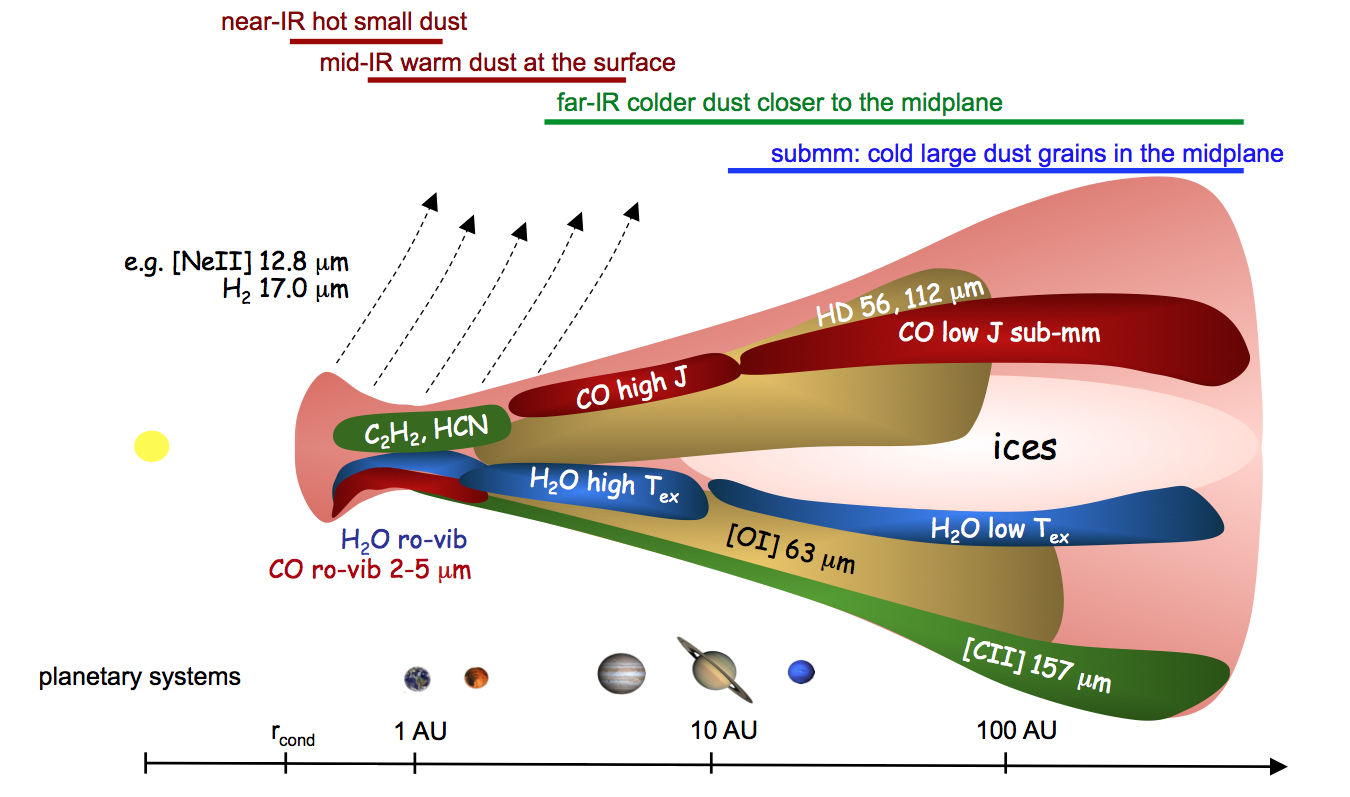
\includegraphics[width=\linewidth]{Figures/disk-sketch.png}
    \caption{A schematic representation of a protoplanetary disk. The planets in the solar system are shown as a point of reference. \cite{inproceedings}}
    \label{fig:enter-label}
\end{figure}

% \section{Radiative Transfer}
\section{Modeling}
Some of the properties of the protoplanetary disks can be directly inferred from disk measurements. For instances where this is not the case, we would still like to learn more from our data via a different method. We can use models to simulate the protoplanetary disk and generate synthetic data to compare to actual observations. There are various types of models. Ranging from 1D slab models to thermo-chemical disk models. For our research, we run simulations using PROtoplanetary DIsk MOdel (Prodimo) a thermo-chemical disk model. The output of those simulations is then put through Fast Line Tracing system (FLiTs) to get an accurate spectrum of the disk. 
% \subsection{ProDiMo}

% \subsection{FLiTs}
\textbf{I still need to figure out how these work so I will add this later}
\chapter{Methods}\label{Ch: Methods}
\section{Data}
For our research, we ran a model grid with 25 models with ProDiMo and used FLiTs to get the spectra. (but I may receive many more)
\textbf{INSERT TABLE OF PARAMETERS}
\section{Analysis}
This part is still unknown as I just received the parts of the data and the project is still really open-ended 
\chapter{Results}
\chapter{Discussion}
\chapter{Conclusion}
\bibliographystyle{lion-msc}
\bibliography{references}

\end{document}